\section{NavCSP experimentation}
Navigating a model adds a great deal of complexity.
The pointer navigation \autoref{csp:nav} is the greatest factor in that complexity.
It takes effect in variable query expressions such as:
\texttt{src.var(ref).prop}
where we want to find a property based on variables in the scope of the solver.
Whether the property is variable or not, or is an attribute or a reference, the same navCSP applies.
In the case the property is a reference, we can chain the CSP, which greatly increases complexity.

\subsubsection{OCL Query Dimensions}
To evaluate the navigation provided by \autoref{csp:nav}, we will look at the size of the CSP modeling the following OCL expression:
$$\texttt{let query = self.ref.ref...ref in}$$
% $$\texttt{query->sum(attrib) = Constant}$$
% $$\texttt{query->isUnique(attrib)}$$
Such that 
% all the references are variable, and
% , and the attributes constant.
% The query has two dimensions which we will vary: reference size $N$, and navigation depth $d$. 
% \texttt{Obj} is an instance of an object.
\texttt{self.ref} is reflexive variable reference, modeled with $N$ pointer variables, identifying objects of the same type.
The depth of the navigation, is noted $d$, with $d=0$ as the case of variable property access, \texttt{query = self.ref}.
Adding further navigations increments $d$, for example $d=2$ corresponds to \texttt{self.ref.ref.ref}.

% We will first outline the size of the constraint model, and with an implementation we will search for a maximum sum to get interesting solutions and times.
\subsubsection{OCL Query Size}
% \ytodo{change the word: hyper-table}
In \autoref{fig:navcount} we can see the number of \emph{query atoms}, meaning equally: the intermediate pointer variables, element constraints or pointer arithmetic required to model this query, which is found using the formula:
% This is also proportional to the number of constraints for navigation, and the number of intermediate variables.
$$f(N,0)=0$$
$$f(N,d)=f(N,d-1)+N^{1+d}$$
\noindent 1) No matter the size of the \texttt{AdjList}, the first annotated reference implies no intermediate pointers, as we simply find the problem variables associated to \texttt{self}.

\noindent 2) If we are to navigate deeper, we make an additional hyper-table of intermediate variables, indexed by the prior lower dimension table of pointers.
% , of which the domains are enforced by an equal number of element constraints.
To examine the formula, let's look at the case of $d=1$, or \texttt{self.ref.ref}:
$$
f(N,1) = 0 + N^{2}
$$

We have N pointers coming in from \texttt{self.ref}, and they each point to N pointers.
% , as seen in \autoref{csp:nav}.
Resulting in a table of intermediate pointer variables.
If we navigate deeper, let  $d=2$:
$$f(N,2) = 0 + N^2 + N^3$$
For every pointer in the previous table $N^2$, we associate N more pointers.
Giving us now a \emph{hyper-table}, cubed.
If we navigate deeper, the 3D hyper-table will similarly index a 4D hyper-table.

% \ytodo{There is a commented figure and intuition into: hyper-tables}
% \begin{figure}[ht]
%     \centering
%     \includegraphics[width=0.5\linewidth]{figures/hypertable.pdf}
%     \caption{visualisation of the hyper-table of problem variable copies indexed by a lower-dimensional table of pointer variables, where N=2, N'=3 and N"=4}
%     \label{fig:hypertable}
% \end{figure}
% In \autoref{fig:hypertable} we have a crude visualisation of a hyper-table indexed by a lower dimensional table, made to line up with $f(N,2)$, but N has been split into N=2, N'=3, and N"=4 to see better.
% We can see the normal square-like table of pointer variables on the left, resulting from the first navigation.
% And on the right, the cube-like hyper-table holding the possible results of the second navigation according to the results of the first.

The graph in \autoref{fig:navcount} starts at 1 on the x,y axes or $f(1,1)$, which gives 1 on the z axis (log scale).
% The z axis is scaled logarithmically to powers of 10.
% One pointer variable x=1, and single navigation y=1, results in a single element constraint.
For a single navigation from a single pointer variable (AdjList of size 1), we have a single query atom. 
For a single navigation from an \texttt{AdjList} of size 10 or $f(10,1)$, we have 100 query atoms. 
For \texttt{AdjList} variables of size 1, navigating with a query depth of 10 or $f(1,10)$, results in 10 query atoms.

On the left background, we can see the curve resulting from increasing \texttt{AdjList} size.
While on the right, we can see the curve resulting from increasing navigation depth.
We can see from this that increasing the navigation seems to increase the size of the problem logarithmically, while increasing the number of pointers for a reference is exponential.


\begin{figure}[ht]
    \centering
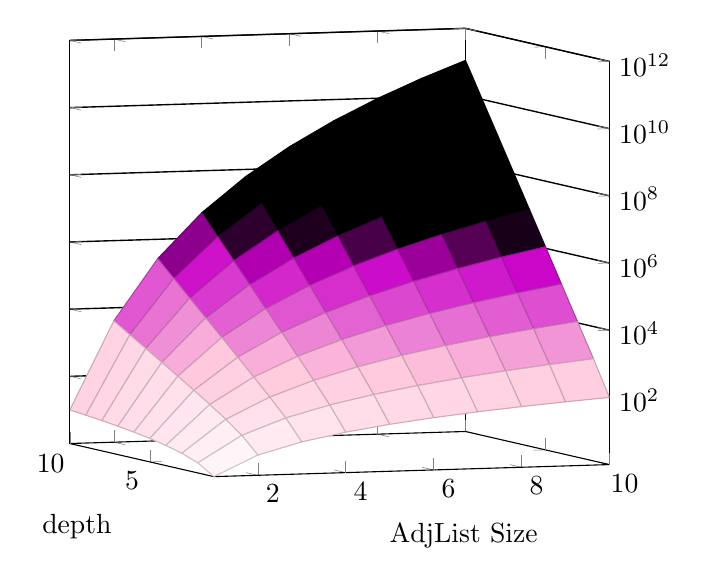
\begin{tikzpicture}
\begin{axis}[
    xlabel={AdjList Size},
    ylabel={depth},
    zmode=log,
    zmin=1e0,
    zmax=1e12,
    zticklabel pos=right,
    ztick={1e2, 1e4, 1e6, 1e8, 1e10, 1e12},
    zmajorgrids=true,
    grid style={line width=0.5pt, draw=black},
    view={-20}{5},
    % colormap name=viridis,
    % shader=interp,
    colormap={custom}{ % Define a custom colormap
        [1cm] 
        color(0cm)=(white) 
        % rgb255(1cm)=(50,255,230)
        % color(1cm)=(cyan)
        rgb255(25cm)=(255,200,220)
        rgb255(50cm)=(200,0,200)
        % color(2cm)=(violet)
        color(59cm)=(black)
        % rgb255(4cm)=(60,20,60)
        % rgb255(5cm)=(100,80,100)
        color(100cm)=(black)}
    ]
\addplot3[surf,] 
coordinates{
(1,1,1) (1,2,2) (1,3,3) (1,4,4) (1,5,5) (1,6,6) (1,7,7) (1,8,8) (1,9,9) (1,10,10) 

(2,1,4) (2,2,12) (2,3,28) (2,4,60) (2,5,124) (2,6,252) (2,7,508) (2,8,1020) (2,9,2044) (2,10,4092) 

(3,1,9) (3,2,36) (3,3,117) (3,4,360) (3,5,1089) (3,6,3276) (3,7,9837) (3,8,29520) (3,9,88569) (3,10,265716) 

(4,1,16) (4,2,80) (4,3,336) (4,4,1360) (4,5,5456) (4,6,21840) (4,7,87376) (4,8,349520) (4,9,1398096) (4,10,5592400) 

(5,1,25) (5,2,150) (5,3,775) (5,4,3900) (5,5,19525) (5,6,97650) (5,7,488275) (5,8,2441400) (5,9,12207025) (5,10,61035150) 

(6,1,36) (6,2,252) (6,3,1548) (6,4,9324) (6,5,55980) (6,6,335916) (6,7,2015532) (6,8,12093228) (6,9,72559404) (6,10,435356460) 

(7,1,49) (7,2,392) (7,3,2793) (7,4,19600) (7,5,137249) (7,6,960792) (7,7,6725593) (7,8,47079200) (7,9,329554449) (7,10,2306881192) 

(8,1,64) (8,2,576) (8,3,4672) (8,4,37440) (8,5,299584) (8,6,2396736) (8,7,19173952) (8,8,153391680) (8,9,1227133504) (8,10,9817068096) 

(9,1,81) (9,2,810) (9,3,7371) (9,4,66420) (9,5,597861) (9,6,5380830) (9,7,48427551) (9,8,435848040) (9,9,3922632441) (9,10,35303692050) 

(10,1,100) (10,2,1100) (10,3,11100) (10,4,111100) (10,5,1111100) (10,6,11111100) (10,7,111111100) (10,8,1111111100) (10,9,11111111100) (10,10,111111111100)
};
\end{axis}
\end{tikzpicture}
\caption{Number of query atoms in relation to \texttt{AdjList} size and navigation depth}
    \label{fig:navcount}
    \Description[AST]{}
\end{figure}


The complete navigation model has twice as many constraints $2f(N,d)$, as we need both an element and some pointer arithmetic for each intermediate variable. 
Our implementation of the pointer arithmetic implies an additional intermediate variable, giving a total of $2f(N,d)$ intermediate variables.
% To quote \cite{jackson_alcoa_2000} the models resulting from the relational logic are \emph{huge}.

The total number of propagations required to find all counter proofs, or validate a model also aligns with the number of constraints found here $2f(N,d)$, validation would correspond to all the problem variables having only one possible value. 
While it is a large number it's still fast to run all these propagators once, and running out of memory space for the model became a more limiting factor than time in our tests.

Going beyond validation, and searching for a model fix, or completing a model such as in our use-case, means increasing the domains of the problem variables and by consequence the intermediate variables, and in the case of model completion having the full range of possibilities for all these variables.

\subsubsection{Subset Sum Problem}\footnote{\url{https://github.com/ArtemisLemon/navCSP_SubsetSum}}
by applying the following constraints to the query from a single object (among up to 120), we can model a variation on the subset sum problem:
$$\texttt{query->sum(attribute) = Target}$$
$$\texttt{and query->isUnique(attribute)}$$
Where \texttt{self.attribute} of an object is a constant integer attribute between 10 and 29. 
All of them together forming a multiset, from which we'll find a subset with the right sum.
Initial testing with this problem gives fast non-trivial solutions, up to a few minutes, for queries with up to around $10^4$ intermediate variables.
When no subset sums equal the target, such as finding a subset summing to 1, or when solving for trivial targets such as 0, the process takes less than a few minutes up to $10^6$ intermediate variables.
% If we were to attempt model repair, we could slightly increase the domain around the disproven values, and search for models in that space, which would be much smaller than in this context.
% Taking in total less than minute for up to $10^5$ intermediate variables.
Bigger problems reached our memory limit.
% Another notable observation, is building the Choco CSP often takes longer than disproving this case. 
% \ytodo{apply to all objects?}
These results color \autoref{fig:navcount}, the lightest area being quickly solvable, the darker area being quickly verifiable and the black area being too big to model.

% The evaluation instance will all follow the same pattern.
% The multisets will be the first M elements of a repeating sequences of $[10..30[$.
% The target sums will be 10 as it will appear in all the multisets, the max subset sum $S=\frac{M}{2}*(10+(10+M-1))$ of a multiset.
% In cases where there is a solution path, those values will be bold?

% To get solutions, we search in the problem variables, here those representing the references, and the variable to which the top most constraint is applied. 